\chapter{安全分析の基本手法: FTAとFMEA}
\label{chap2}
\section{未然防止の手法}
障害への対応法は、応急処置、再発防止、および未然防止がある。応急処置、再発防止は発生した障害に対応する事後解析であり、リアクティブな方法(Reactive Approach)と呼ばれる。未然防止は、障害が発生してから対策を取るのではなく、計画段階や設計段階の生産の源流において、将来起こりうる障害を洗い出して、それらに対策を講じてしまうことである。潜在的な障害に対応する事前解析であり、プロアクティブな方法(proactive approach)といわれる。未然防止の手法には、FMEA(Failure Mode and Effect Analysis), FTA(Fault Tree Analysis), ETA(Event Tree Analysis), 良品解析などがある。信頼性工学や安全性工学では良さ加減を増強するよりも、悪さ加減を減少させる方法がとられることが多い。

未然防止技術は多くある(多変量解析、品質機能展開、品質工学、実験計画法、WCA、FEM、信頼性試験、故障解析、信頼性データ解析、リスク・アセスメント、ライフサイクル・アセスメント(LCA))。本講義では、最も代表的なFTA, FMEAを扱う。
\section{FTAとFMEA}
 FMEA, FTAは対象とするシステム(製品、設備、プロセスなど)の故障、不具合、欠陥などの「悪さ加減」を論理的に洗い出して、内在する問題点を発見する解析手法である。見出された問題点に対しては、実際の技術活動や管理活動を通じて対策や是正措置が取られる。
 
FTAとFMEAの形態を示す。図\ref{191}、図\ref{192}は、工作用の洋ばさみについてのFTAとFMEAである。
\begin{figure}[htbp]
\begin{center}
%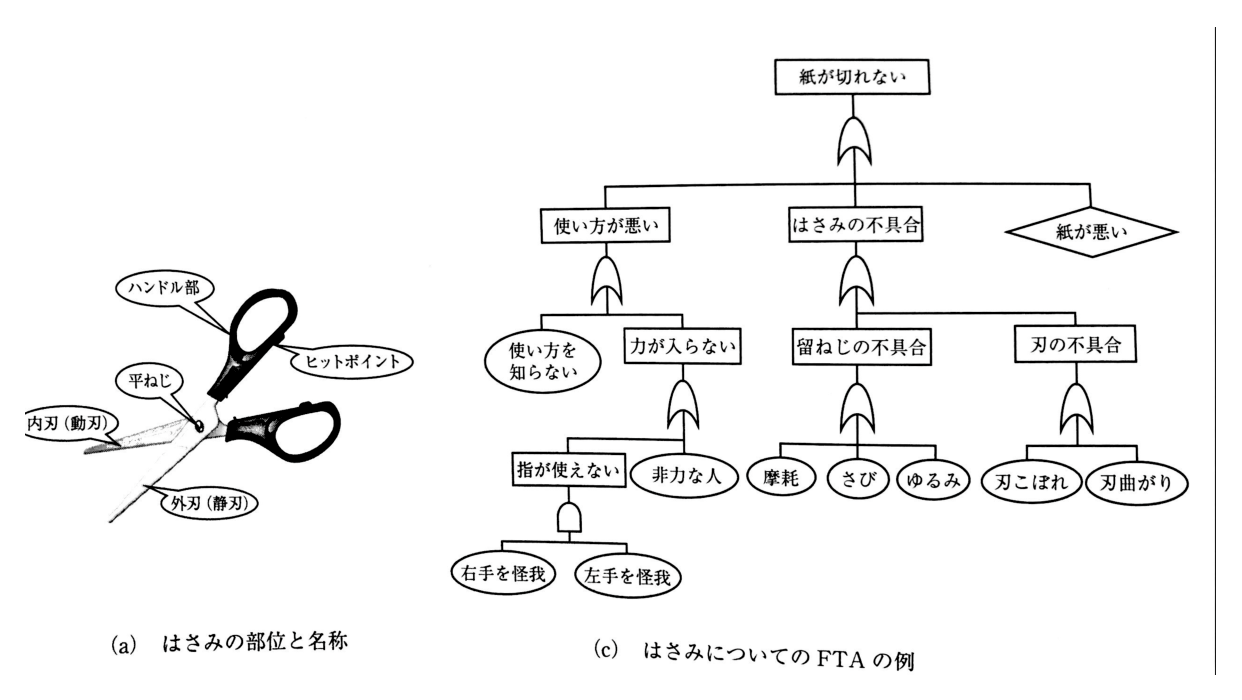
\includegraphics[width=15cm]{safety_assurance_contents/ch2images/191}
\end{center}
\caption{FTAの形態(工作用はさみの事例)}
\label{191}
\end{figure}
(a)ははさみの部分と名称を示したもので、内刃、外刃、留ねじの3つの部品からなる。(b)ははさみに対して実施した設計FMEAを示す。部品の故障モードを洗い出して、システム(この場合ははさみ)への影響を表形式で解析する手法である。原因系から結果系を予測する方法と言える。
\begin{figure}[htbp]
\begin{center}
%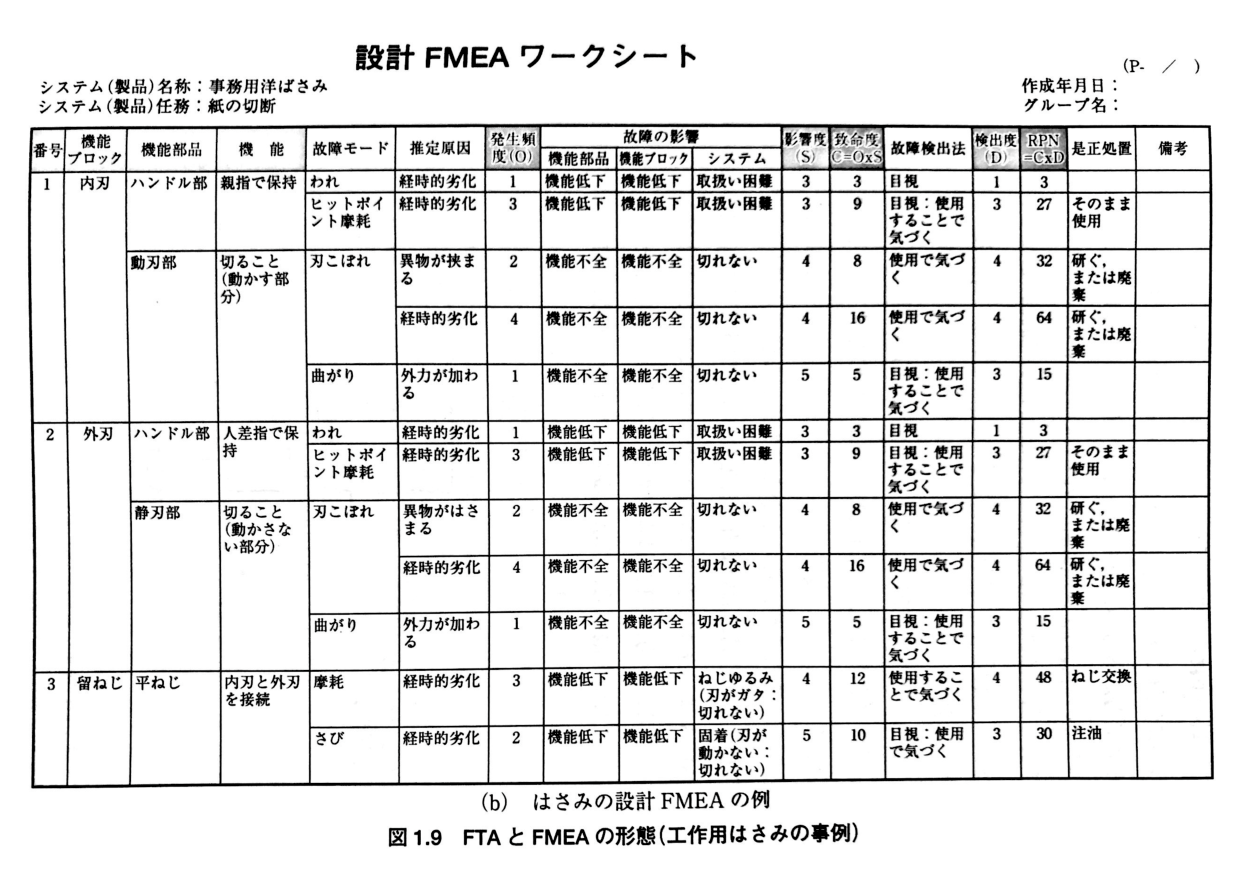
\includegraphics[width=15cm]{safety_assurance_contents/ch2images/192.eps}
\end{center}
\caption{FMEAの形態(工作用はさみの事例)}
\label{192}
\end{figure}
(c)は、はさみで紙が切れないという結果の事象を取り上げて、その原因を探るFTAの一部を示す。FTAは木構造の解析手法である。主な論理ゲートはANDゲート(論理積)とORゲート(論理和)である。

一般にシステムはサブシステムに、サブシステムはコンポーネントに、というように、順次、下位の構成要素に分解される。最終的にこれ以上分解できないレベルにいたる。システムとしては、階層的に分解できる構造であれば、ハードウエアでも、ソフトウエアでも、プロセスでも、あるいはそれらの複合でもよい。FMEAは下位の階層の悪さ加減が上位の階層の悪さ加減にどのように影響するかを表形式上で論理的に解析する手法である。FTAは逆に上位の階層の悪さ加減の原因となる下位の階層の悪さ加減を木構造で論理的に解析する手法である。FMEAは単一の原因が及ぼす複数の結果を網羅的に洗い出すのに優れた手法であるが、複数の原因によって及ぼされる結果の洗い出しは難しい。一方、FTAは複数の原因によって及ぼされる結果も表現できるが、網羅性が十分ではない。両者は相補的かつ相乗的に用いられている。
\section{FTA(Fault Tree Analysis、故障の木解析)}
FTAは、「なぜなぜ」を繰り返すことで、重大な故障やトラブルの発生要因を下方に向かって木構造として展開し、網羅した要因の中から重要な要因を抽出する。1979年にスリーマイル島で発生した原子力事故の解析の際、マサチューセッツ工科大学教授のRasmussenが原因の特定に使用したことでその有効性が評価され広まった手法である。
\subsection{FT図を読む}
FT図は、視覚的に故障に至るメカニズムが大変わかりやすく表現されている。FT図の記号は、イベントを示す事象記号と、それらの間の因果関係を示す論理記号とに分けられる。表\ref{43}にある4つの記号の意味を理解できれば、ほとんどのFT図を読むことができる。
\begin{table}[htbp]
\caption{FTAで用いる基本的な記号}
\begin{center}
%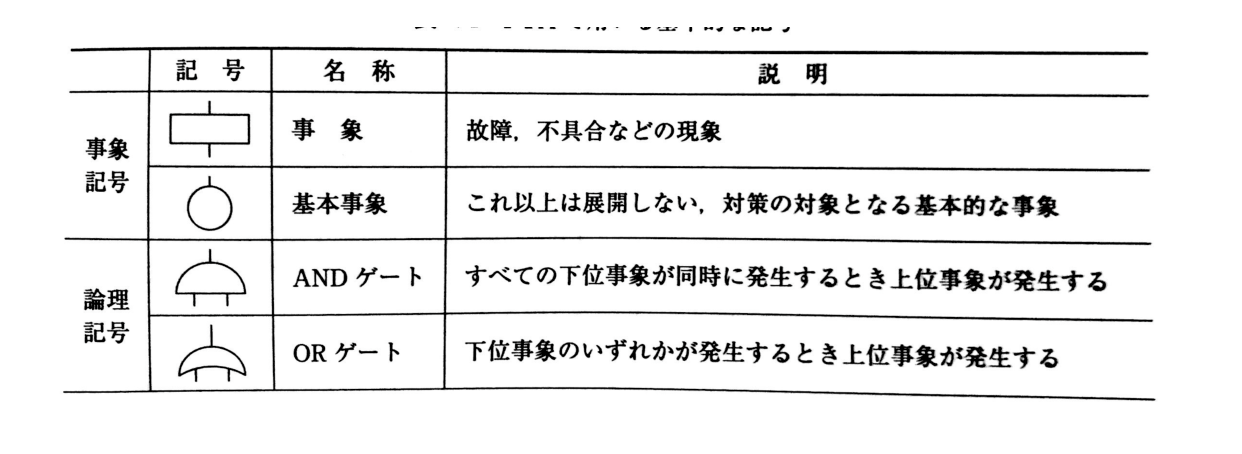
\includegraphics[width=13cm]{safety_assurance_contents/ch2images/44.eps}
\end{center}
\label{43}
\end{table}
さらに、表\ref{44}のノードも用いられる。
\begin{table}[htbp]
\caption{FTAで用いる便利な記号}
\begin{center}
%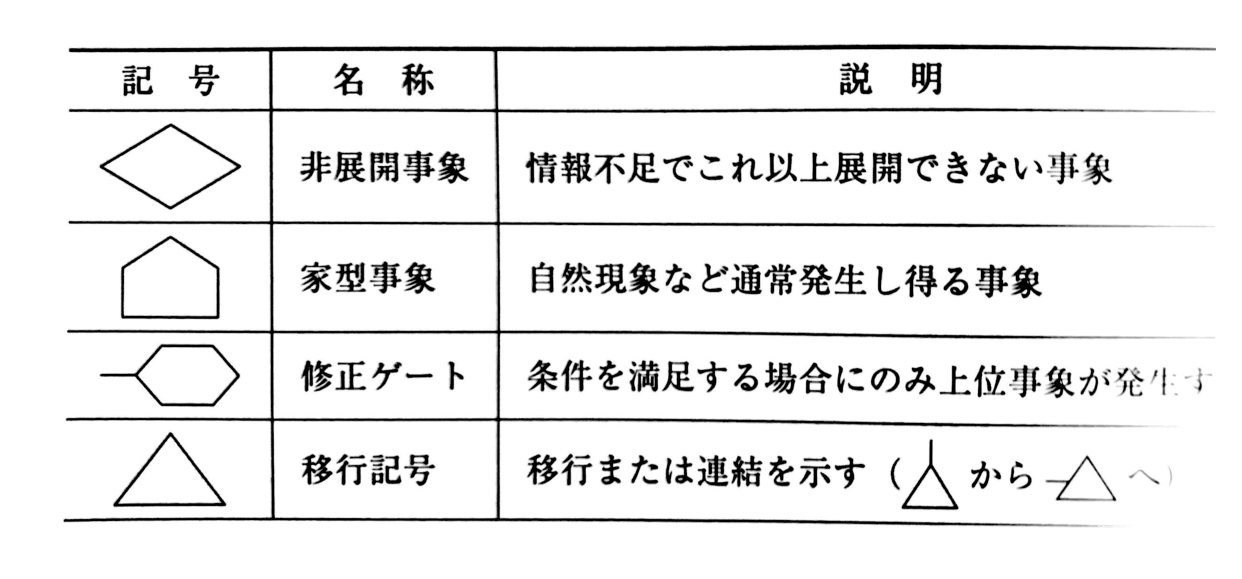
\includegraphics[width=11cm]{safety_assurance_contents/ch2images/45.eps}
\end{center}
\label{44}
\end{table}
FT図の例を図\ref{415}に示す。トップ事象である欠報の原因には「火災の検知信号が届かない」不具合と「ブザーが鳴らない」不具合とがあり、いずれか一方の原因で欠報に陥ることが示されている。さらに、その2つ以外に原因がないこと、あるいは他の原因は無視してよいことを示している点が重要である。この必要十分性は、熟練者でもしばしば見落とす点である。一方のANDゲートは、すべての下位事象が同時に発生するときに上位事象が発生することを示す記号で、並列型に対応する。「火災の検知信号が届かない」事象は、冗長に設置された2つのセンサ系A,Bが同時に故障しているときのみ発生する事象となる。
\begin{figure}[htbp]
\begin{center}
%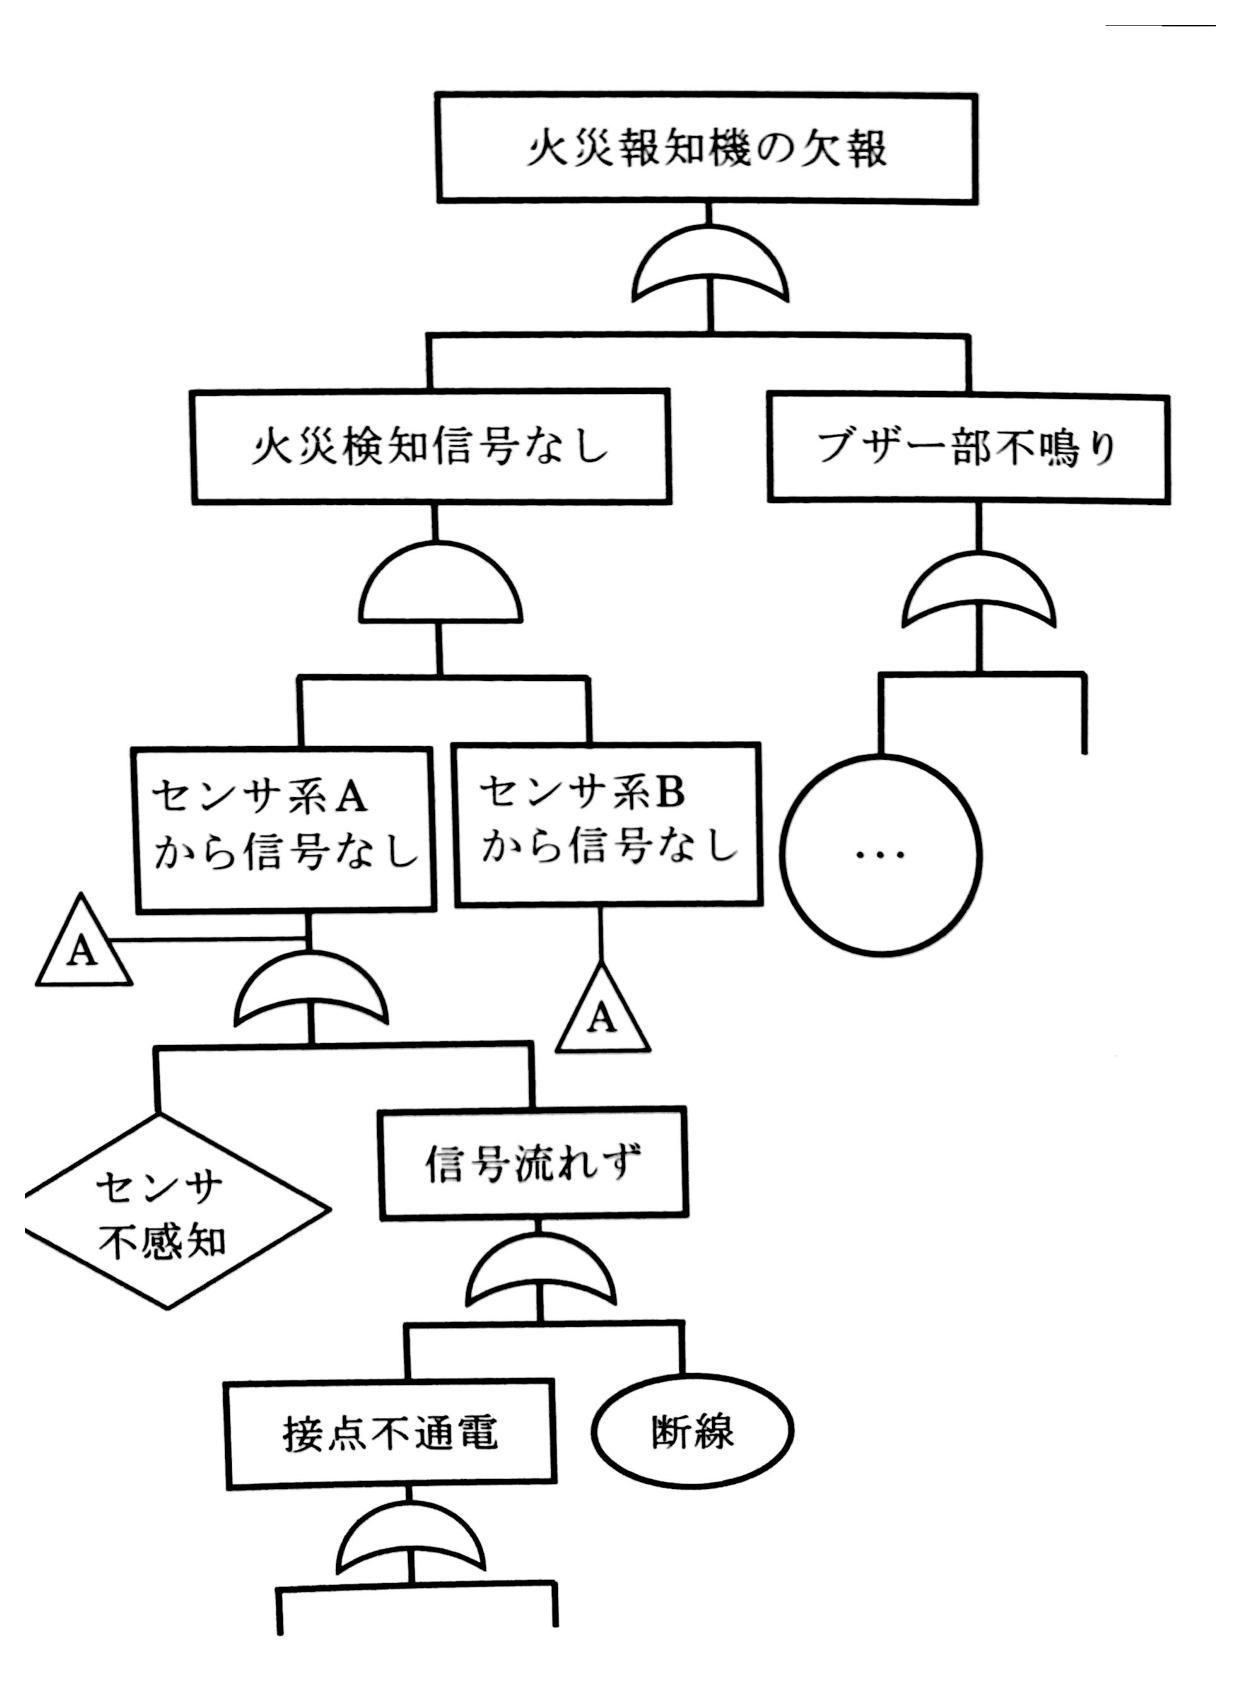
\includegraphics[width=7cm]{safety_assurance_contents/ch2images/145.eps}
\end{center}
\caption{FT図の例}
\label{415}
\end{figure}
FTAには、
\begin{itemize}
\item トップ事象と基本事象との因果関係が視覚的に示され、多様な事象間関係を把握しやすい。
\item ANDゲートにより多重故障を解析できる。
\end{itemize}
などの特徴がある。
\subsection{FT図の作成}
FTAの実施は、FT図の作成とFT図の解析の2つのステップで構成される。ここでは作成までの手順を説明する。
\begin{enumerate}
\item FTA実施の準備。対象製品を熟知する技術者と品質保証担当者を含めた3名から6名程度のメンバーで実施する。設計資料、図面、材料部品リストや想定使用状況、関連するトラブル、クレーム情報、特に不具合に関する情報を集める。
\item 解析対象の機能の理解。FTAで解析する対象製品の構造や機能について、参加者全員で十分理解する。自分の専門とする部分や分野に対象を限定することなく、周辺との関係なども理解することが重要である。
\item トップ事象の選定。信頼性や安全性を損なうような「発生することが望ましくない」トップ事象を注意深く選定する。その際、1. 明確に定義できる事象、2. 多くの下位事象の結果として発生する事象、3. 設計の中で技術的に対処できる基本事象が予想される事象、であることが望ましい。1が最も重要な要件であり、「明確」なとは、その事象発生の有無の判断が人によって異なることはない、との意味である。例えば「エアバッグが開かない(不動作故障)」、「エアバッグが不要のときに開く(誤作動故障)」などは、トップ事象としてふさわしい。しかし「***の満足度が低い」、「***の回転が不安定」などは、その範囲(基準値)が不明瞭であり適さない。また一見良さそうに見える「排気ガス規制の基準値を満たしていない」のような表現も避けるべきである。ガスの種類や基準値は時代と共に変化するので、「排気ガスCOの規制基準値**ppmを満たさない」などの具体的な基準値を明記する必要がある。2.は、FTA解析はマンパワーが必要となるので、できるだけ重要なトップ事象を扱う、という意味である。3.は、設計時に、FT図作成に関わる技術者が基本事象まで書ききることができるようにするためである。
\item トップ事象の1次要因への展開。トップ事象の1次要因を、製品の構造や機能、手順1で準備した情報などを基に列挙し、論理記号を用いて因果関係を明確に図示する。

展開する方法は大きく分けて2つある。
\begin{enumerate}
\item 構造(信頼性ブロック図)からの作成。あるシステムが信頼性ブロック図で構造が示される場合、直列系の部分をORゲートに、並列型部分をANDゲートに対応させることで、FT図を容易に作成できる。
\item 機能を考えて作成。実際には、信頼性ブロック図を基にFT図全てを作成できるケースは多くない。構成要素の機能に着目して、トップ事象の直接の原因である1次要因を抽出し、さらにそれらの原因である2次要因を抽出するという具合に、意味を考えてトップダウンに作成することになる。
\end{enumerate}
1次要因への展開は、最も頭を悩ませるステップだが、重要な箇所であり、時間をかけるべき手順である。システムを構成するサブシステムごとに空間的に分割し、それぞれを解析するとの方針がとられることが多いが、それよりも、エネルギーの流れに注目するなど、機能的な側面から1次要因を分解すると、装置間の相互作用などを見失うことが少なく、効果的な木になることが多い。
\item トップ事象の2次要因以下への展開。展開可能な1次要因に関して、さらになぜなぜ分析を続け、2次要因、3次要因を列挙、基本事象または非展開事象に至るまで論理記号を用いて展開する。
\end{enumerate}
例題 図\ref{41}に示されるような、2つのセンサが並列に設置された自動照明器で、「照明が点灯しない」をトップ事象とするFT図を作成せよ。
\begin{figure}[htbp]
\begin{center}
%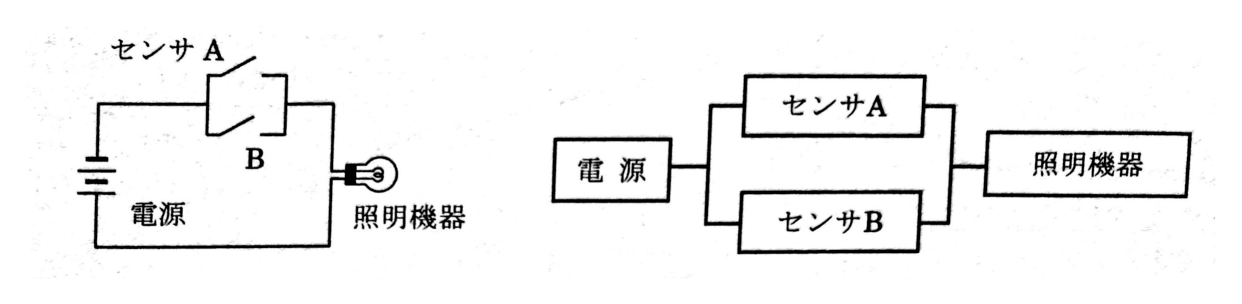
\includegraphics[width=10cm]{safety_assurance_contents/ch2images/41.eps}
\end{center}
\caption{照明設備の回路図と信頼性ブロック図}
\label{41}
\end{figure}


\section*{参考文献}
本資料は「システムの信頼性と安全性、田中健次、朝倉書店」、「新FMEA技法、益田昭彦、高橋正弘、本田陽広、日科技連」を基にしている。
